\documentclass[12pt]{article}
\usepackage{homework}
\pagestyle{fancy}

% assignment information
\def\course{Electromagnetism}
\def\assignmentno{Problem Sheet 3}
\def\assignmentname{Electromagnetic Waves}
\def\name{Xin, Wenkang}
\def\time{\today}

\begin{document}

\begin{titlepage}
    \begin{center}
        \large
        \textbf{\course}

        \vfill

        \Huge
        \textbf{\assignmentno}

        \vspace{1.5cm}

        \large{\assignmentname}

        \vfill

        \large
        \name

        \time
    \end{center}
\end{titlepage}


%==========
\pagebreak
\section*{Electromagnetic Waves}
%==========


\problem{3.1}{Poynting vector and resistance heating}

\subproblem{a}
For a cylindrical resistor supplied with a potential difference $V$, the electric field inside is uniform:

\begin{equation}
    \mathbf{E} = \frac{V}{L} \hat{z}
\end{equation}

where $\hat{z}$ is the unit vector along the direction of current.

The magnetic field is given by Ampere's law:

\begin{equation}
    \mathbf{B} = \frac{\mu_{0} I}{2\pi r} \hat{\phi}
\end{equation}

\subproblem{b}
The Poynting vector is given by:

\begin{equation}
    \mathbf{S} = \frac{1}{\mu_{0}} \mathbf{E} \times \mathbf{B} = -\frac{VI}{2\pi aL} \hat{r}
\end{equation}

which gives the total power flowing into the resistor:

\begin{equation}
    P = \int_{S} \mathbf{S} \cdot (-\hat{r}) \mathrm{d}S = VI
\end{equation}

which is expected from Joule heating.

\subproblem{c}
Outside the wire, the magnetic field is circumferential with $B = \hat{\phi} \mu_{0} I/2\pi r$. The electric field is produced by the battery and is such that the Poynting vector points into the resistor.
\qed


\problem{3.2}{Standing wave and radiation pressure}

\subproblem{a}
Consider the reflected wave:

\begin{equation}
\begin{split}
    \tilde{\mathbf{E}}_{R} &= E_{0,R} e^{i(-kx - \omega t)} \hat{x} \\
    \tilde{\mathbf{B}}_{R} &= -B_{0,R} e^{i(-kx - \omega t)} \hat{y}
\end{split}
\end{equation}

and the transmitted wave:

\begin{equation}
\begin{split}
    \tilde{\mathbf{E}}_{T} &= E_{0,T} e^{i(\kappa x - \omega t)} \hat{x} \\
    \tilde{\mathbf{B}}_{T} &= B_{0,T} e^{i(\kappa x - \omega t)} \hat{y}
\end{split}
\end{equation}

where $\kappa^{2} = \mu \epsilon \omega^{2} + i\mu \sigma$ is the complex wave number of the transmitted wave.

Demanding that the parallel components of the electric and magnetic fields are continuous at $z = 0$ gives:

\begin{equation}
\begin{split}
    E_{0} + E_{0, R} = E_{0, T} \\
    \frac{1}{\mu_{0}} (B_{0} - B_{0, R}) = \frac{1}{\mu_{0}} B_{0, T}
\end{split}
\end{equation}

The magnetic fields are related to the electric fields by $B = E/v$ where $v$ is the speed of light in the medium. Solving the equations for $E_{0, T}$ gives:

\begin{equation}
    E_{0, T} = \frac{2}{1 - \mu_{0}c/\mu v} E_{0}
\end{equation}

where $v = \omega/\kappa$ is the complex velocity of the transmitted wave.

For a perfect conductor, we have $\sigma \to \infty$ so $\kappa \to \infty$ and $v \to 0$. The transmitted wave is then zero and the reflected wave has the amplitude:

\begin{equation}
    E_{0, R} = -E_{0}
\end{equation}

\subproblem{b}
In the $z<0$ region, the net fields are:

\begin{equation}
\begin{split}
    \tilde{\mathbf{E}} &= E_{0} \left[ e^{i(kz - \omega t)} - e^{i(-kz - \omega t)} \right] \hat{x} = 2i E_{0} \sin{(kz)} e^{-i\omega t} \hat{x} \\
    \tilde{\mathbf{B}} &= B_{0} \left[ e^{i(kz - \omega t)} + e^{i(-kz - \omega t)} \right] \hat{y} = 2 B_{0} \cos{(kz)} e^{-i\omega t} \hat{y}
\end{split}
\end{equation}

Thus, the nodal planes for the electric field are at $z = n\pi/k$ and the nodal planes for the magnetic field are at $z = (n+1/2)\pi/k$ for $n \in \mathbb{Z}$. This is characteristic of a standing wave.

\subproblem{c}
The Poynting vector is given by:

\begin{equation}
    \mathbf{S} = \frac{1}{\mu_{0}} \mathbf{E} \times \mathbf{B} = 2i \frac{E_{0}^{2}}{\mu_{0}c} \sin{(2kz)} e^{-2i\omega t} \hat{z}
\end{equation}

which is zero at the nodal planes.

The energy `oscillates' between nodal planes. The time average of the Poynting vector is:

\begin{equation}
    \left\langle \mathbf{S} \right\rangle = \sqrt{2} \frac{E_{0}^{2}}{\mu_{0}c} \sin{(2kz)}
\end{equation}

\subproblem{d}
The energy density is given by:

\begin{equation}
    u = \frac{1}{2} \left( \epsilon_{0} E^{2} + \frac{B^{2}}{\mu_{0}} \right) = \epsilon_{0} E^{2} = 4 \epsilon_{0} E_{0}^{2} \sin^{2}{(kz)}
\end{equation}

which is equal to its time average as it does not have a time dependence.

\subproblem{e}
There is no surface charge on the conductor as there is no discontinuity in the electric field in the perpendicular direction (zero in both regions).

Consider the displacement current caused by the incident electric field:

\begin{equation}
    \mathbf{J}_{D} = \left. \epsilon_{0} \frac{\partial \tilde{\mathbf{E}_{i}}}{\partial t} \right|_{z=0} = -i\omega \epsilon_{0} E_{0} e^{-i\omega t} \hat{x}
\end{equation}

Consider a ribbon of width $\delta y$ lying perpendicular to the x-axis. The surface current is given by:

\begin{equation}
    \mathbf{K} = -i\omega \epsilon_{0} E_{0} e^{-i\omega t} \delta y \hat{x}
\end{equation}

so that the magnetic field due to the displacement current is:

\begin{equation}
    -i\omega \epsilon_{0} E_{0} e^{-i\omega t} \delta y \frac{\mu_{0}}{2} \hat{y}
\end{equation}
\qed


\problem{3.3}{Fresnel's formulas}

\subproblem{a}
At the boundary, we need continuous parallel components of the electric fields:

\begin{equation}
    \tilde{\mathbf{E}}_{i} + \tilde{\mathbf{E}}_{r} = \tilde{\mathbf{E}}_{t}
\end{equation}

This equation must hold for $z = 0$ and all $t$. Hence, the exponential terms must be equal, leading to:

\begin{equation}
    \mathbf{k}_{i} \cdot \mathbf{r} = \mathbf{k}_{r} \cdot \mathbf{r} = \mathbf{k}_{t} \cdot \mathbf{r}
\end{equation}

which must hold at $z = 0$.

We can choose $\mathbf{r} = (1, 0, 0)$ so that the above equation becomes:

\begin{equation}
    k_{i} \sin{\theta_{i}} = k_{r} \sin{\theta_{r}} = k_{t} \sin{\theta_{t}}
\end{equation}

Since the incident and reflected waves are in the same medium, we have $k_{i} = k_{r}$ and $\theta_{i} = \theta_{r}$, which is the law of reflection. The other equality gives Snell's law:

\begin{equation}
    \frac{\sin{\theta_{i}}}{\sin{\theta_{t}}} = \frac{k_{t}}{k_{i}} = \frac{v_{t}}{v_{i}} = n
\end{equation}

where we define the (relative) refractive index $n$ as the ratio of the speed of light in the two media.

If $n < 1$, there will exist some $\theta_{i} = \theta_{ic} = \arcsin{(n)}$ such that the transmitted wave will be evanescent for $\theta_{i} > \theta_{ic}$. This is also known as total internal reflection.

\subproblem{b}
For perpendicular polarisation, we impose the continuity of the parallel components of the electric and magnetic fields:

\begin{equation}
\begin{split}
    E_{i, 0} - E_{r, 0} &= E_{t, 0} \\
    \frac{1}{\mu_{0}} \cos{\theta_{i}} (B_{i, 0} + B_{r, 0}) &= \frac{1}{\mu_{0}} \cos{\theta_{t}} B_{t, 0}
\end{split}
\end{equation}

Since the magnetic fields are related to the electric fields by $B = E/v$, we can solve the above equations for $E_{t, 0}$ and $E_{r, 0}$:

\begin{equation}
\begin{split}
    \tilde{E}_{t, 0} &= \frac{2 \cos{\theta_{i}}}{\cos{\theta_{i}} + n\cos{\theta_{t}}} E_{i, 0} = \frac{2}{1 + \alpha n} E_{i, 0} \\
    \tilde{E}_{r, 0} &= \frac{\cos{\theta_{i}} - n\cos{\theta_{t}}}{\cos{\theta_{i}} + n\cos{\theta_{t}}} E_{i, 0} = \frac{1 - \alpha n}{1 + \alpha n} E_{i, 0}
\end{split}
\end{equation}

where we define $\alpha = \cos{\theta_{t}}/\cos{\theta_{i}} = \sqrt{1 - \sin^{2}{\theta_{i}}/n^{2}}/\cos{\theta_{i}}$.

The reflection coefficient is given by:

\begin{equation}
    R = \left\lvert \frac{\tilde{E}_{r, 0}}{\tilde{E}_{i, 0}} \right\rvert^{2} = \left( \frac{1 - \alpha n}{1 + \alpha n} \right)^{2}
\end{equation}

\begin{figure}[ht]
    \centering
    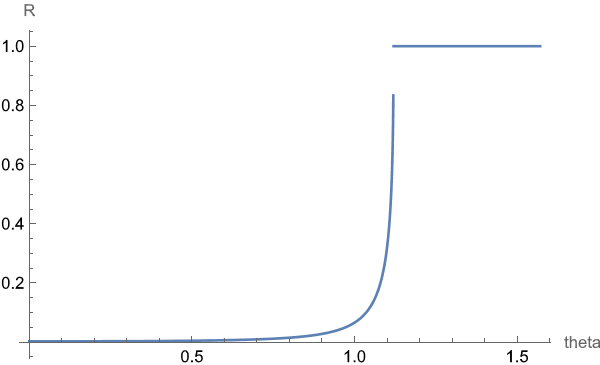
\includegraphics[width=0.5\textwidth]{../plots/electro_3_3_a.png}
    \caption{Reflection coefficient for $n = 0.9$.}
    \label{fig:reflection_coefficient_1}
\end{figure}

\begin{figure}[ht]
    \centering
    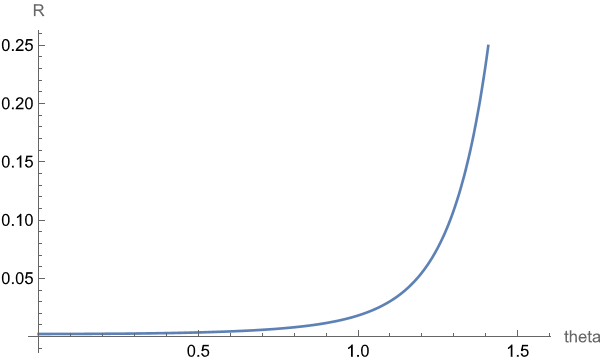
\includegraphics[width=0.5\textwidth]{../plots/electro_3_3_b.png}
    \caption{Reflection coefficient for $n = 1.1$.}
    \label{fig:reflection_coefficient_2}
\end{figure}

\subproblem{c}
For parallel polarisation, we still impose the boundary conditions:

\begin{equation}
\begin{split}
    (E_{i, 0} + E_{r, 0}) \cos{\theta_{i}} &= E_{t, 0} \cos{\theta_{t}} \\
    \frac{1}{\mu_{0}} (B_{i, 0} - B_{r, 0}) &= \frac{1}{\mu_{0}} B_{t, 0}
\end{split}
\end{equation}

Solving for $E_{t, 0}$ and $E_{r, 0}$ gives:

\begin{equation}
\begin{split}
    \tilde{E}_{t, 0} &= \frac{2}{n + \alpha} E_{i, 0} \\
    \tilde{E}_{r, 0} &= \frac{n - \alpha}{n + \alpha} E_{i, 0}
\end{split}
\end{equation}

Note that there now exists an angle for which there is not reflected wave. To achieve this, let $n = \alpha$ so that $\cos{\theta_{t}}/\cos{\theta_{i}} = n$. This is Brewster's angle.

The reflection coefficient is given by:

\begin{equation}
    R = \left\lvert \frac{\tilde{E}_{r, 0}}{\tilde{E}_{i, 0}} \right\rvert^{2} = \left( \frac{n - \alpha}{n + \alpha} \right)^{2}
\end{equation}

\begin{figure}[htt]
    \centering
    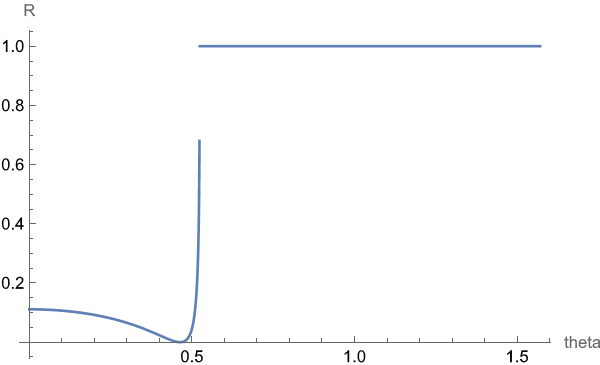
\includegraphics[width=0.5\textwidth]{../plots/electro_3_3_c.png}
    \caption{Reflection coefficient for $n = 0.5$.}
    \label{fig:reflection_coefficient_3}
\end{figure}

\begin{figure}[htt]
    \centering
    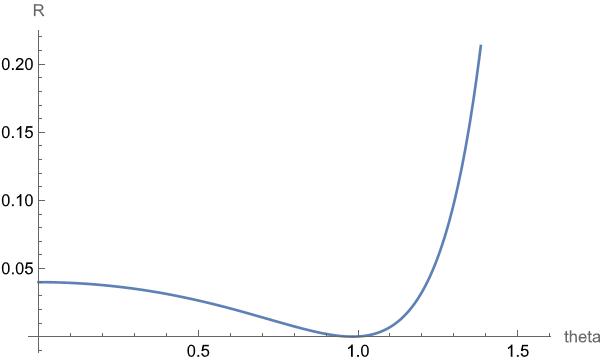
\includegraphics[width=0.5\textwidth]{../plots/electro_3_3_d.png}
    \caption{Reflection coefficient for $n = 1.5$.}
    \label{fig:reflection_coefficient_4}
\end{figure}

\subproblem{d}
At Brewster's angle, we have:

\begin{equation}
    \sin{\theta}_{i} \cos{\theta_{t}} = \sin{\theta}_{t} \cos{\theta_{i}}
\end{equation}

which gives $\sin{2\theta_{i}} = \sin{2\theta_{t}}$. 

Since $\theta_{i} \ne \theta_{t}$, we must have $\theta_{i} + \theta_{t} = \pi/2$ at Brewster's angle. This means that the dipoles are oscillating in such a direction that is perpendicular to reflected wave. Hence, there is no reflected wave.
\qed


\problem{3.4}{Waves in the ionosphere}

\subproblem{a}
For a plasma, the equation of motion of the electrons is:

\begin{equation}
    m_{e} \ddot{x} = -\frac{e^{2}n_{e}}{\epsilon_{0}} x - eE
\end{equation}

where $E = E_{0} e^{-i\omega t}$ is some oscillating external electric field.

The plasma frequency is defined as:

\begin{equation}
    \omega_{p} \equiv \sqrt{\frac{e^{2}n_{e}}{m_{e} \epsilon_{0}}}
\end{equation}

The particular solution is:

\begin{equation}
    x = \frac{e}{m_{e} \omega^{2}} E_{0} e^{-i\omega t}
\end{equation}

On the other hand, this displacement creates a polarisation:

\begin{equation}
    P = \frac{p_{tot}}{V} = -e n_{e} x = \epsilon_{0} (\epsilon_{r} - 1) E
\end{equation}

where at the last equality we have used the definition of the relative permittivity $\epsilon_{r}$.

Solving for $\epsilon_{r}$ gives:

\begin{equation}
    \epsilon_{r} = 1 - \frac{\omega_{p}^{2}}{\omega^{2}}
\end{equation}

The dispersion relation is then:

\begin{equation}
    \frac{\omega}{k} = \frac{c}{n} = \frac{c}{\sqrt{\epsilon_{r}}}
\end{equation}

The refractive index may be complex if $\omega < \omega_{p}$, in which case the wave is evanescent.

\subproblem{b}
For $\omega > \omega_{p}$, the refractive index is real and the wave is propagating. For parallel polarisation, we have:

\begin{equation}
    \tilde{E}_{t, 0} = \frac{2}{n + \alpha} E_{i, 0}
\end{equation}

so that total internal reflection occurs when $\alpha$ is complex. For this to occur, we must have $\sin{\theta}_{i} > n$ or:

\begin{equation}
    \theta_{i} > \sin^{-1}{\left( \sqrt{1 - \frac{\omega_{p}^{2}}{\omega^{2}}} \right)}
\end{equation}

For perpendicular polarisation, we have:

\begin{equation}
    \tilde{E}_{t, 0} = \frac{1 - \alpha n}{1 + \alpha n} E_{i, 0}
\end{equation}

which gives the same condition for total internal reflection by setting $\alpha$ to be complex.

\subproblem{c}
Assuming that we can treat the ground as flat, the incident angle $\theta$ and the height of the ionosphere $h$ are related by:

\begin{equation}
    \tan{\theta_{crit}} = \frac{D/2}{h}
\end{equation}

where $D$ is the distance between the transmitter and the receiver.

For critical angle, we must have:

\begin{equation}
    \theta_{crit} = \tan^{-1}{\left( \frac{D/2}{h} \right)} = \sin^{-1}{\left( \sqrt{1 - \frac{\omega_{p}^{2}}{\omega^{2}}} \right)}
\end{equation}

Since $\omega$ is given by the relation $\omega = 2\pi c/\lambda$, we have:

\begin{equation}
\begin{split}
    1 - \frac{\omega_{p}^{2}}{\omega^{2}} &= \sin^{2}{\theta_{crit}} \\
    \omega_{p}^{2} &= \omega^{2} \cos^{2}{\theta_{crit}} \\
    n_{e} &= \frac{\epsilon_{0} m_{e} \omega^{2}}{e^{2}} \cos^{2}{\theta_{crit}}
\end{split}
\end{equation}

Evaluating, we have $n_{e} = \qty{2.5e6}{cm^{-3}}$ which is comparable to the maximum F layer density during daytime.

\subproblem{d}
For signals with frequency $\omega \gg \omega_{p}$, we have a refractive index approximately equal to $1$. This means that the ionosphere is transparent to these signals so the signals propagate into space and are not reflected back to the ground. Signals with lower frequencies can be reflected back to the ground. Aiming for the ionosphere can help increase the range of the signal and avoid obstacles on the ground.

\subproblem{e}
At night, there is less UV present to ionise the atmosphere so $n_{e}$ is lower. This means a lower $\omega_{p}$ and higher refractive index. In the end, there is a lower $\theta_{crit}$ required for total internal reflection so that farther distances can be reached.
\qed


\problem{3.5}{Waves in a good conductor}

\subproblem{a}
In a conductor, we have the Maxwell equations:

\begin{equation}
\begin{split}
    \nabla \cdot \mathbf{E} &= \frac{\rho_{f}}{\epsilon_{0}} \\
    \nabla \cdot \mathbf{B} &= 0 \\
    \nabla \times \mathbf{E} &= -\frac{\partial \mathbf{B}}{\partial t} \\
    \nabla \times \mathbf{B} &= \mu_{0} \mathbf{J} + \mu_{0} \epsilon_{0} \frac{\partial \mathbf{E}}{\partial t}
\end{split}
\end{equation}

For a good conductor, any free charges are quickly distributed. Hence, $\rho_{f} = 0$. We also have $\mathbf{J} = \sigma \mathbf{E}$ for an Ohmic conductor. Taking the curl of the last equation gives:

\begin{equation}
    \nabla^{2} \mathbf{E} = \mu_{0} \epsilon_{0} \frac{\partial^{2} \mathbf{E}}{\partial t^{2}} + \mu_{0} \sigma \frac{\partial \mathbf{E}}{\partial t}
\end{equation}

which is a modified wave equation that admits the plane wave solution:

\begin{equation}
    \tilde{\mathbf{E}} = \tilde{\mathbf{E}}_{0} e^{i(\kappa z - \omega t)}
\end{equation}

where the complex wave number $\kappa$ is given by:

\begin{equation}
    \kappa^{2} = \mu_{0} \epsilon_{0} \omega^{2} + i \mu_{0} \sigma \omega = \mu_{0} \epsilon_{0} \omega^{2} \left( 1 + i \frac{\sigma}{\epsilon_{0} \omega} \right)
\end{equation}

Comparing this with the wave number in vacuum $k^{2} = \mu_{0} \epsilon_{0} \omega^{2}$, we see that the complex dielectric constant can be written as:

\begin{equation}
    \tilde{\epsilon}_{r} = 1 + i \frac{\sigma}{\epsilon_{0} \omega}
\end{equation}

We can also write the wave number as $\kappa = k_{+} + ik_{-}$ where:

\begin{equation}
    k_{\pm} = \omega \frac{\sqrt{\mu_{0} \epsilon_{0}}}{2} \left( \sqrt{1 + \frac{\sigma^{2}}{\epsilon_{0}^{2} \omega^{2}}} \pm 1 \right)^{1/2} = \frac{\omega}{2c} \left( \sqrt{1 + \frac{\sigma^{2}}{\epsilon_{0}^{2} \omega^{2}}} \pm 1 \right)^{1/2}
\end{equation}

Replacing $\omega$ with $2/(\mu_{0} \sigma \delta^{2})$, we have:

\begin{equation}
    k_{\pm} = \frac{1}{c \mu_{0} \sigma \delta^{2}} \left( \sqrt{1 + \frac{\mu_{0}^{2} \sigma^{4} \delta^{4}}{4\epsilon_{0}^{2}}} \pm 1 \right)^{1/2} \approx \frac{1}{c \mu_{0} \sigma \delta^{2}} \left( \sigma \delta \sqrt{\frac{\mu_{0}}{2\epsilon_{0}}} \right) = \frac{1}{\delta}
\end{equation}

The dispersion relation is then:

\begin{equation}
    \frac{\omega}{k_{+}} = v
\end{equation}

where $v$ is the phase velocity of the wave.

Differentiating the dispersion relation with respect to $\omega$ gives:

\begin{equation}
    \frac{v_{g}}{v} = \frac{\mathrm{d}\omega/\mathrm{d}k_{+}}{\omega/k_{+}} = 1 + \frac{\sigma^{2}}{\sigma^{2} + 8\epsilon_{0}^{2} c^{2} k_{+}^{2}} \approx 2
\end{equation}

where the approximation is valid for $\sigma \gg \omega \epsilon_{0}$.

The dispersion is anomalous because the group velocity is twice the phase velocity.

We can write the electric and magnetic fields as:

\begin{equation}
\begin{split}
    \tilde{\mathbf{E}} &= \tilde{E}_{0} e^{-k_{-} z} e^{i(k_{+} z - \omega t)} \hat{x} \\
    \tilde{\mathbf{B}} &= \frac{\kappa}{\omega} \tilde{E}_{0} e^{-k_{-} z} e^{i(k_{+} z - \omega t)} \hat{y}
\end{split}
\end{equation}

so that the impedance is given by:

\begin{equation}
    Z = \frac{E_{0}}{B_{0}/\mu_{0}} = \frac{\mu_{0}\omega}{\kappa} = \frac{\mu_{0}\omega\delta}{(1 + i)} = \frac{1 - i}{\delta \sigma}
\end{equation}

\subproblem{b}
The Poynting vector is given by:

\begin{equation}
    \mathbf{S} = \frac{1}{\mu_{0}} \tilde{\mathbf{E}} \times \tilde{\mathbf{B}} = \frac{1 + i}{2} \delta \sigma \tilde{E}_{0}^{2} e^{-2k_{-} z} e^{2i(k_{+} z - \omega t)} \hat{z}
\end{equation}

which has the time average:

\begin{equation}
    \left\langle \mathbf{S} \right\rangle = \frac{1}{2} \delta \sigma \tilde{E}_{0}^{2} e^{-2k_{-} z} \hat{z}
\end{equation}

\subproblem{c}
The energy density is given by:

\begin{equation}
    u = \frac{1}{2} \left( \epsilon_{0} E^{2} + \frac{B^{2}}{\mu_{0}} \right)
\end{equation}

For the electric part, we have:

\begin{equation}
    \left\langle \frac{1}{2} \epsilon_{0} E^{2} \right\rangle = \frac{1}{2} \epsilon_{0} \tilde{E}_{0}^{2} e^{-2k_{-} z}
\end{equation}

For the magnetic part, we have:

\begin{equation}
    \left\langle \frac{1}{2\mu_{0}} B^{2} \right\rangle = \frac{\left\lvert \kappa \right\rvert^{2}}{2\mu_{0} \omega^{2}} \tilde{E}_{0}^{2} e^{-2k_{-} z} = \frac{1}{\mu_{0} \omega^{2} \delta^{2}} \tilde{E}_{0}^{2} e^{-2k_{-} z} = \frac{\sigma}{2\omega} \tilde{E}_{0}^{2} e^{-2k_{-} z}
\end{equation}

which shows that the energy is mainly stored in the magnetic field.

The total time-averaged energy density is then:

\begin{equation}
    \left\langle u \right\rangle = \frac{1}{2} \epsilon_{0} \tilde{E}_{0}^{2} e^{-2k_{-} z} + \frac{\sigma}{2\omega} \tilde{E}_{0}^{2} e^{-2k_{-} z} = \frac{1}{2} \epsilon_{0} \tilde{E}_{0}^{2} e^{-2k_{-} z} \left( 1 + \frac{\sigma}{\epsilon_{0} \omega} \right)
\end{equation}

The velocity of energy flow is given by:

\begin{equation}
    \frac{\left\lvert \left\langle \mathbf{S} \right\rangle \right\rvert}{\left\langle u \right\rangle} = \frac{\delta \sigma}{\epsilon_{0} (1 + \sigma/\epsilon_{0} \omega)} \approx \delta \omega = v
\end{equation}

which is just the phase velocity of the wave.
\qed


\end{document}